\documentclass[12pt]{article}
\usepackage[a4paper, margin=1in]{geometry}

\usepackage{amsmath}
\usepackage{mathtools}
\usepackage{amssymb}
\usepackage{hyperref}
\usepackage{graphicx}

\title{Internship Report}
\date{March 9, 2025}
\author{Aanjishnu Bhattacharyya}

\begin{document}

\maketitle

\section*{Introduction}

Numerical Analysis is an very important part of mathematics. It provides us with the tools nessesary to tackle
real-life math problems which are hard to solve analytically. Functions such as the gamma functions and the normal
distribution are extremely difficult to calculate analytically and sometimes impossible. Improper Integrals and
integrals of higher dimentional functions may also be solved in a efficient manner utilizing these methods.

We have tried to build a simple yet powerful software utility which is able to integrate functions with vector valued
inputs and vector valued outputs. It is possible to have multiple nested integrals with varying limits including improper
integrals. Simpsons and Trapezoidal methods are used since they provide a good compromise speed and correctness.
The software utility also provids a rudimentary 3-d visualization framework to plot relevant functions utilizing 3d-acceleration 
hardware present in most modern computers. The software utility also utilizes the feature of runtime link libraries
provided by most modern operating system to provide a seameless user experience.

\section*{Learning Phase}

In the learning phase we first develop the mathematical background required for this task.

\subsection*{Numerical Method of calculating Integrals}

To compute the integrals of any function, we must first consider the problem of approximating the function.
Approximation in this context reffers to the reconstruction of a function from $n$ sampled points obtained
from the function. This problem becomes much simpler if the sample points are spaced equally apart from eachother.
Fortunately in our particular case we have direct access the the function itself thus it is trivial to obtain such
points. Simpsons method and Trapezoidal method perform the best under these given constraints.
\break
\break

\begin{align*}
	\text{Let, } \quad &f : \mathbb{R} \rightarrow \mathbb{R}\\
			   &f_i = f(x_i) \qquad \forall x_i \in \mathbb{R} \quad \wedge \quad 0 \le i \le n\\\\
	\text{Let, } \quad &L : \mathbb{R} \rightarrow \mathbb{R}\\
		    &L(x) = \sum_{i=0}^n \omega^n_i(x) f_i\\
	&\omega^n_i(x) = \prod \limits_{\substack{j=0 \\ i \not = j}}^n \frac{x - x_j}{x_i - x_j}& \quad i \not = j\\\\
	\text{Now, } \quad &I = \int_{a}^{b} f(x) \mathrm{d}x \qquad \qquad a = \min\{x_i\} \wedge b = \min\{x_i\}\\
				    &= \int_{a}^{b} L(x) \mathrm{d}x\\
				    &= \int_{a}^{b} \sum_{i=0}^n \omega^n_i(x) f_i \mathrm{d}x\\
				    &= \sum_{i=0}^n \int_{a}^{b} \omega^n_i(x) f_i \mathrm{d}x\\
				    &= \sum_{i=0}^n f_i \int_{a}^{b} \prod \limits_{\substack{j=0 \\ i \not = j}}^n \frac{x - x_j}{x_i - x_j} \mathrm{d}x\\\\
	\text{Let, } \quad &h = x_i - x_{i - 1} \qquad \qquad \because x_i\text{ is equispaced}\\
			   &u = \frac{x - x_0}{h}\\
			   &\mathrm{d}u = \frac{1}{h} \mathrm{d}x\\\\
	\text{Substituting }u, \quad &\\
				   &= \sum_{i=0}^n f_i \int_{0}^{n} h \prod \limits_{\substack{j=0 \\ i \not = j}}^n \frac{u - j}{i - j} \mathrm{d}u\\
				   &= \sum_{i=0}^n f_i \frac{h \cdot -1^{n-i}}{i! \cdot (n-i)!} \int_{0}^{n} \prod \limits_{\substack{j=0 \\ i \not = j}}^n {(u - j)} \mathrm{d}u  &\text{\small{(1)}}
\end{align*}

\break
From this general formulae we can derive equations for both Simpsons $(n=2)$ and Trapezoidal $(n=1)$ rules,

\begin{align*}
	\text{From \small{(1)}, } \quad\\
	&I = \sum_{i=0}^n f_i \frac{h \cdot -1^{n-i}}{i! \cdot (n-i)!} \int_{0}^{n} \prod \limits_{\substack{j=0 \\ i \not = j}}^n {(u - j)} \mathrm{d}u\\\\
	\text{For n = 1,}\\
	&= \sum_{i=0}^1 f_i \frac{h \cdot -1^{1-i}}{i! \cdot (1-i)!} \int_{0}^{1} \prod \limits_{\substack{j=0 \\ i \not = j}}^1 {(u - j)} \mathrm{d}u\\\\
	&= -f_0 \cdot h \cdot \int_0^1 (u - 1) \mathrm{d}u + f_1 \cdot h \cdot \int_0^1 u \mathrm{d}u\\
	&= -f_0 \cdot h \cdot \left[ \frac{u^2}{2} - u \right]_0^1 + f_1 \cdot h \cdot \left[\frac{u^2}{2} \right]_0^1\\
	&= (f_0 + f_1) \frac{h}{2}\\\\
	\text{For n = 2,}\\
	&= \sum_{i=0}^2 f_i \frac{h \cdot -1^{2-i}}{i! \cdot (2-i)!} \int_{0}^{2} \prod \limits_{\substack{j=0 \\ i \not = j}}^2 {(u - j)} \mathrm{d}u\\\\
	&= f_0 \cdot h \cdot \int_0^1 (u - 1)(u - 2) \mathrm{d}u - f_1 \cdot h \cdot \int_0^1 u(u - 2) \mathrm{d}u\\
	& \qquad\qquad\qquad\qquad+ f_2 \cdot h \cdot \int_0^1 u(u - 1) \mathrm{d}u\\
	&= (f_0 + 4f_1 + f_2) \frac{h}{3}\\
\end{align*}

\subsection*{Integrals with improper limits}

Integrals with improper limits can often be broken down into subpieces which can be computed separately.

e.g,
\begin{equation*}
	\int_{-1}^1 \frac{1}{x} \mathrm{d}x = \lim_{z \rightarrow 0} \left( \int_{-1}^{z} \frac{1}{x} \mathrm{d}x + \int_{z}^{1} \frac{1}{x} \mathrm{d}x \right)
\end{equation*}

We can also have limits which have infinities as their limits, in these cases we can construct a series with
the integrals themselves and try to understand if the series converges. If it does we can also compute for what
values.

e.g,
\begin{equation*}
	\int_{0}^\infty e^{-x^2} \mathrm{d}x\\
\end{equation*}

Let us consider the series,
\begin{equation*}
	S_n = \int_{0}^n e^{-x^2} \mathrm{d}x\\
\end{equation*}

We can say $S_k$ converges if at a large enough value of $k$ equals $S_{k+1}$ given a particular precision.
\begin{equation*}
	S_{n+1} - S_{n} < \vert \epsilon \vert \quad \quad n \ge k \in \mathbb{R}
\end{equation*}

\subsection*{Computing Multiple Integrals}

Multiple integrals to compute the volumes and other higher dimentional constructs can be computed through the same methods.
Computing the limits from the outer most integral and then computing limits for these integrals from the inner most integral.
How ever on of the many contrains of this system requires that each limit be defined as a function instead of conditional constraint,
and it may be nesessary to convert conditional constraints into limits

e.g,
\begin{align*}
	&\iint \limits_{x^2 + y^2 \le r^2} f(x, y) \mathrm{d}A\\
	= &\int_{-r}^{r} \left( \int_{-\sqrt{r^2 - y^2}}^{\sqrt{r^2 - y^2}} f(x, y)\mathrm{d}x \right) \mathrm{d}y
\end{align*}

\section*{Training}

\subsection*{Building an simple prototype of a function integrator and plotter.}

We build a simple prototype in javascript to understand how we should aproach building the integrator software \ref{fig:prototype1}.
During this process we avoid using several built in features and external libraries of javascript as to undestand
the internals of such a system and also to keep the program as light weight as possible.

The prototype was capable of integrating any function whose domain was $\mathbb{R}^2$ and range was $\mathbb{R}$.
The interface developed in this prototype resembled that of graphing software desmos. The major things that we learned
from building this prototype were:
\begin{itemize}
	\item The computation time increased rapidly with decrease in the magnitude of $h$ so it was imperative that
		we language which does not have a very high overhead.

	\item We need to separate out the graphing part of the program from the computation part to make it effective and
		fast.

	\item We must allow the user to input data in a known syntax, and allow them to edit the functions at runtime.
\end{itemize}

\begin{figure}
	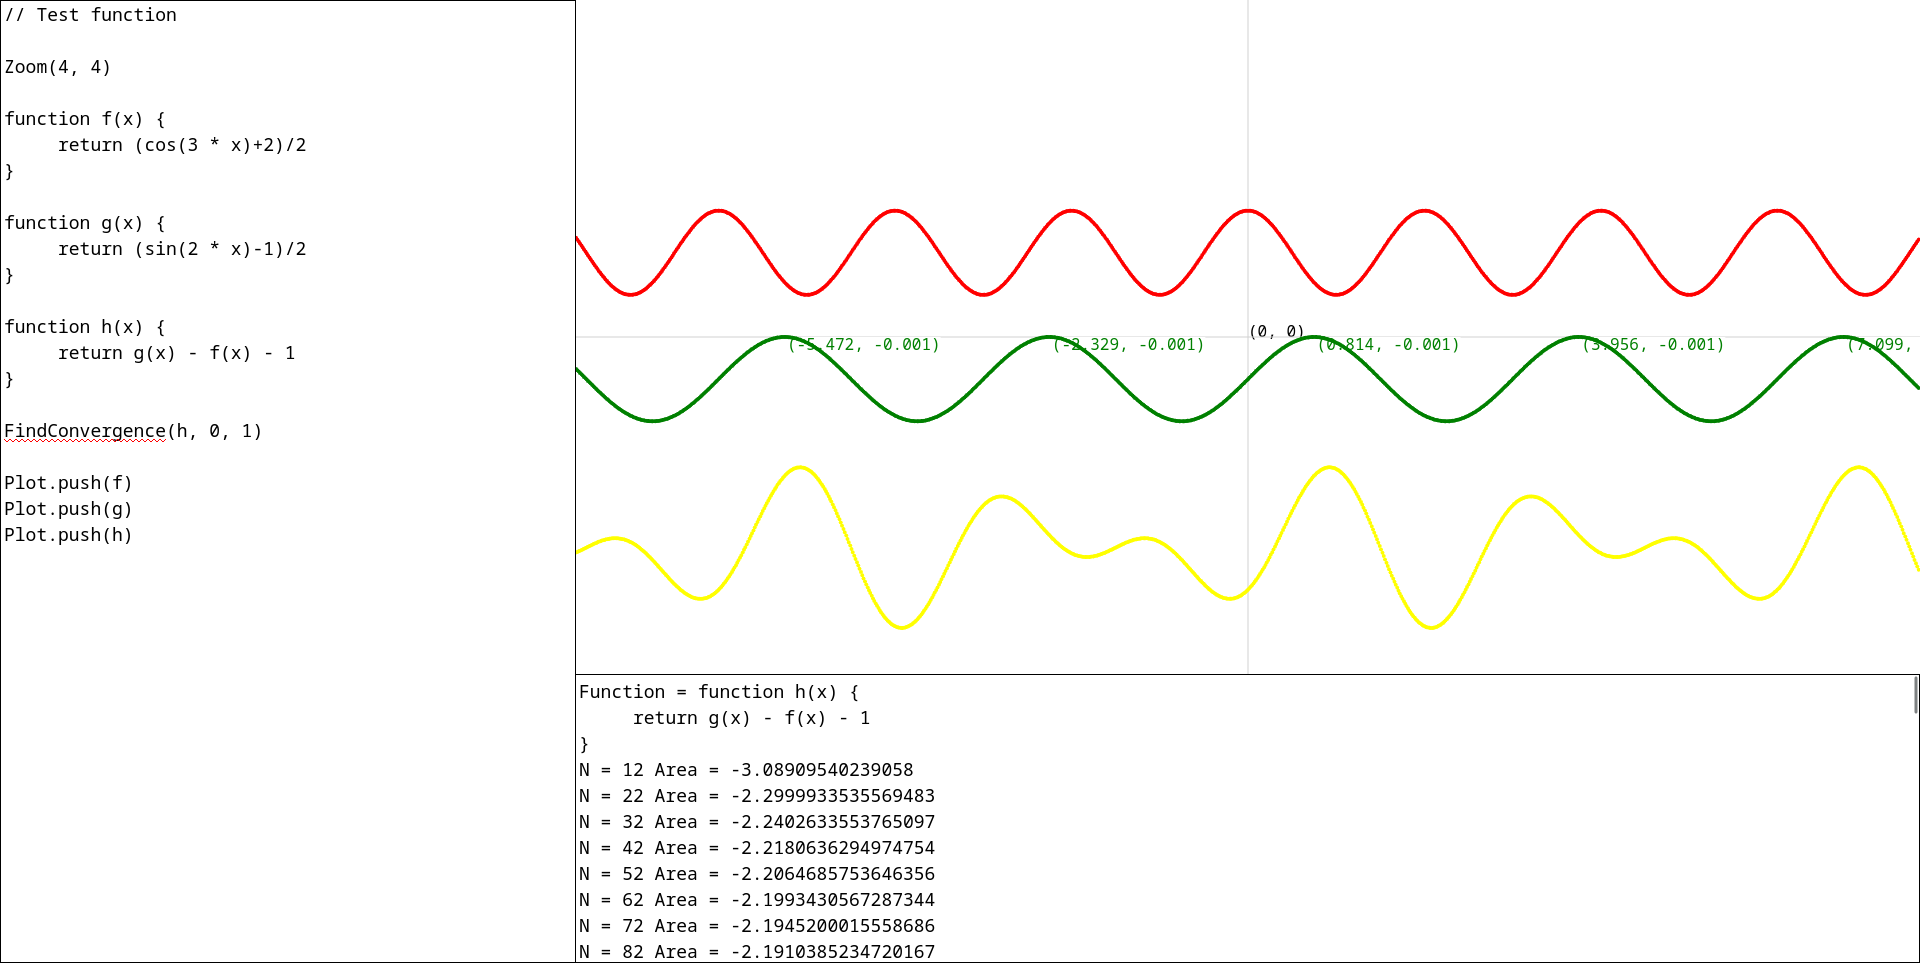
\includegraphics[width=\linewidth]{prototype.png}
	\caption{Integrating and plotting a trigonometric function}
	\label{fig:prototype1}
\end{figure}

It is possible to access the prototype from any computer via the internet at: \url{https://nimcompoo-04.github.io/numlysis} 


\section*{Project}
%\section*{Results}
%\section*{Conclusion}

\end{document}
